\documentclass[fleqn,10pt]{wlscirep}
\usepackage[utf8]{inputenc}
\usepackage[T1]{fontenc}
\usepackage{amsmath,amssymb}
\usepackage{array,booktabs,tabularx}
\usepackage{graphicx}
\usepackage{float}
\usepackage{algorithm}
\usepackage{algpseudocode}
\usepackage{lineno}
\usepackage{microtype}
\usepackage{url}
\usepackage{seqsplit}

\newcolumntype{Y}{>{\raggedright\arraybackslash}X}
\newcolumntype{L}[1]{>{\raggedright\arraybackslash}p{#1}}
\DeclareRobustCommand{\code}[1]{\path{#1}}
\newcommand{\Rank}{\operatorname{rank}}
\newcommand{\tok}{\operatorname{token}}
\newcommand{\Enc}{\operatorname{Enc}}
\newcommand{\Dec}{\operatorname{Dec}}
\modulolinenumbers[5]

\title{RankCloak: Hiding Synthetic Cryptographic Artifacts in Plain English with Language Models}

\author[1,*]{Alexander V. Mantzaris}
\affil[1]{School of Data, Mathematical, and Statistical Sciences, University of Central Florida, Orlando, FL, United States of America}
\affil[*]{Correspondence: alexander.mantzaris@ucf.edu}

\keywords{linguistic steganography, large language models, rank transcoding, exact-copy replay, neural steganalysis}

\begin{abstract}
RankCloak transcodes synthetic cryptographic artifacts into natural language using language-model next-token ranks (leveraging an LLM) and realizes those ranks as generated cover text. We compare direct subword representation with bounded ASCII-byte and hex-nibble codecs, including non-segmented generation and segmented forced spans followed by non-payload natural tails. The completed evaluation used 480 public deterministic artifacts from eight cryptographic classes, three open-source model families, and 18 English prompt templates. The secondary recovery tests used Spanish and Simplified Chinese prompts. All 6,480 primary payload trials recovered the serialized payload under saved-token exact-copy replay (Wilson 95\% confidence interval, 0.999408-1.000000), and all 576 multilingual trials recovered under the same condition. This mapping contract has restrictions that visible-text detokenization and retokenization recovered 61.1\% and normalization and formatting changes reduced recovery further. Using markdown transfer, paraphrase, and cross-model decoding recovered none. Automated readability diagnostics were protocol-dependent and are not human produced ratings. Neural detectors strongly distinguished RankCloak covers from the controls (matched ROC-AUC 0.990190 for TextCNN and 0.999834 for DeBERTa-v3-base), providing adverse evidence for concealment. RankCloak therefore provides a reproducible framework for measuring rank pressure, capacity, replay requirements, cover cost, and detectability. It does not establish a secure or deployment-ready covert channel.
\end{abstract}

\begin{document}
\maketitle
\linenumbers
\raggedbottom

\section*{Introduction}\label{sec:introduction}

Generative language models provide a new medium for text steganography because a prompt can define a next-token distribution and a topic direction in which generated text appears. In the Calgacus rank-transcoding construction\cite{NorelliBronstein2026Calgacus}, a sender tokenizes an arbitrary hidden text, records each token's context-dependent rank, and generates a cover text by selecting the correspondingly ranked tokens under a shared cover prompt; the receiver reverses these steps under the same contexts. Calgacus thereby transcodes one hidden-text token into one cover-text token. RankCloak retains that rank-transfer mechanism but also maps exact serialized cryptographic artifacts through direct-subword and bounded codecs, for which payload and cover token counts need not equal the Calgacus baseline. This mechanism connects classical work on covert channels, information-theoretic steganography, information hiding, and provably secure steganography\cite{Simmons1984Prisoners,Cachin1998InformationTheoretic,Hopper2002ProvablySecureSteganography,Petitcolas1999InformationHidingSurvey} with neural and LLM-based linguistic steganography, where hidden information is embedded through choices made during language generation\cite{Fang2017GeneratingSteganographicTextLSTMs,Yang2019RNNStega,Ziegler2019NeuralLinguisticSteganography,DaiCai2019NearImperceptible,Shen2020SelfAdjustingArithmetic,Zhang2021ProvablySecureGenerative,Wang2025DAIRStega,Wu2024GenerativeTextSteganographyLLM,Lin2024ZeroShotGLS}. Related work on LLM watermarking also treats token selection as a carrier of hidden signals, although watermarking is usually aimed at attribution or detection rather than arbitrary payload recovery\cite{Kirchenbauer2023WatermarkLLM}.

A long-running goal in this area is to make arbitrary, encrypted, or otherwise high-entropy data appear as ordinary communication. Early mimic-function work used statistical source models and inverse compression ideas to generate outputs with distributional properties similar to a target source\cite{Wayner1992MimicFunctions,Wayner1995StrongTheoreticalSteganography}. Hiding the Hidden and related linguistic-steganography systems transformed ciphertext into innocuous natural-language text that could later be transformed back into the original ciphertext\cite{ChapmanDavida1997HidingHidden,Bennett2004LinguisticSteganography}. Other text methods carried bits through synonym choice or contextual word substitution\cite{ChangClark2014PracticalLinguisticSteganography}, while network-camouflage systems generalized a similar objective to protocol formats by making encrypted traffic resemble allowed or innocuous traffic\cite{Weinberg2012StegoTorus,Dyer2013FormatTransformingEncryption}. RankCloak follows this same broad goal in an LLM setting. Instead of using a fixed grammar, synonym table, or protocol template, it uses the token choices made by a shared language model. The payload is first converted into ranks, and the cover prompt determines which English tokens occupy those ranks at each step. This also makes the method useful as a measurement tool since it exposes how a hidden artifact changes rank pressure, generated text quality, and the traces available for later detection.

This measurement focus also has defensive value for detecting the presence of such hidden encodings. If hashes, nonces, UUID-like values, or ciphertext strings are carried by generated tokens rather than displayed in their original syntax, surface scanners cannot rely only on visible hexadecimal, base64, UUID, or credential-shaped patterns. Detection must therefore look for indirect evidence, such as low-probability forced tokens, tokenizer artifacts, formatting fragments, unusually regular token choices, segmentation patterns, or differences between payload-bearing spans and non-payload continuations. Covert-channel and stegomalware surveys emphasize that hiding the existence of communication creates detection, capacity-limitation, and countermeasure problems across text and network media\cite{Zander2007CovertChannelsCountermeasures,Badar2025StegomalwareSurvey}. Text steganalysis and generated-text detection work similarly shows that statistical, neural, graph-based, and probability-based features can reveal some generated or steganographic text, while also showing that robust detection is setting-dependent and vulnerable to distribution shift or paraphrase\cite{Wen2019CNNTextSteganalysis,Wu2021GNNLinguisticSteganalysis,Wang2023FewShotLinguisticSteganalysis,Gehrmann2019GLTR,Mitchell2023DetectGPT,Sadasivan2025AIDetection}. The same issue is relevant to AI-safety monitoring, where hidden message passing and secret collusion among agents have been studied as ways that generated text might evade oversight\cite{Motwani2024SecretCollusion,Zolkowski2026EarlySigns}. RankCloak therefore treats hiding and detection as two sides of the same measurement problem: a useful methodology should recover payloads under declared exact-copy conditions while also producing transparent features, controls, and failure modes for steganalysis.

RankCloak proposes a methodology for a specific case: hiding synthetic cryptographic artifacts in generated English text. The payload classes resemble values commonly encountered in security, including hashes, authentication tags, nonces, identifiers, ciphertexts, and signatures\cite{NIST2015SecureHashStandard,Josefsson2006RFC4648,DavisPeabodyLeach2024RFC9562}. These strings are challenging payloads for rank transcoding because they are not natural-language messages. Direct subword tokenization can represent them compactly, but the resulting payload tokens may occupy low-probability positions in the model's next-token distribution\cite{Sennrich2016SubwordUnits,KudoRichardson2018SentencePiece}. A cover generator forced to select such tokens can preserve exact recoverability under matched replay while producing public text with visible artifacts or unusual statistical features. RankCloak gives an approach by which a hash-like string can be carried by generated cover tokens rather than shown as hexadecimal characters. The main methodological development of this paper is that cryptographic-artifact payloads can be treated as representations to be measured, not merely as strings to be passed through an LLM tokenizer. RankCloak therefore compares direct subword rank measurement with bounded-rank payload codecs, including ASCII-byte fixed-radix encodings and a hex-nibble encoding for lowercase hex-like payloads. This design makes the capacity--quality trade-off explicit: direct subword ranks can be short but may impose large rank pressure, whereas bounded encodings constrain the allowed rank range while increasing the number of generated cover tokens. This representation view also separates payload recovery from public-message quality. RankCloak keeps the cover-side model, tokenizer, prompt family, deterministic rank-ordering rule, and replay procedure fixed while varying payload-side encodings and protocol variants. Non-segmented variants emit one cover token per payload rank under a single prompt context. Segmented variants split a payload into short rank chunks, emit payload-bearing forced spans across multiple public messages, and append non-payload natural tails after those forced spans. Because tails do not carry payload ranks, RankCloak reports forced-span and full-message quality proxies separately.

The resulting evaluation introduces RankCloak as a reproducible methodology for measuring how synthetic cryptographic artifacts can be represented as bounded rank sequences and expressed as LLM-generated cover text under exact-copy replay. The study is organized around how artifact-like payloads affect rank pressure, how bounded encodings change capacity and cover length, and how segmentation and natural tails change the relationship between payload-bearing spans and full messages. Exact-copy replay remains the supported recovery condition, so the sender and receiver must share the same model artifact, tokenizer, prompt rendering, filtering, deterministic configuration, codec, boundaries, and generated token identifiers. This condition is consistent with recent work showing that tokenization and retokenization mismatches can disrupt LLM-based steganography and watermarking\cite{YanMurawaki2025TokenizationInconsistency}. Visible-text detokenization and retokenization is a separate, weaker recovery condition. The expanded evaluation spans public cryptographic test vectors, prompt and model families, and secondary-language conditions, and examines robustness, detectability, automated readability diagnostics, capacity, and computational overhead. RankCloak's contribution is therefore a controlled methodology for hiding and measuring synthetic cryptographic artifacts while making representation, recovery, cover-quality, and detection trade-offs explicit; it does not establish practical robustness, security, undetectability, or human-perceived naturalness.

\section*{Methods}\label{sec:methods}

RankCloak measures whether serialized artifacts that do not normally look like language can be represented as language-model token ranks and then expressed as generated cover text while remaining exactly recoverable under a declared replay contract. Conceptually, the method proceeds in four steps. First, the payload is converted into a sequence of integer ranks. Second, a cover prompt defines the next-token ordering used for public-text generation. Third, the sender emits the token at each required rank under that cover context. Fourth, the receiver replays the same context and recovers the rank of each received token. The non-segmented procedure maps one payload to one cover sequence; the segmented procedure maps a hexadecimal payload to several ordered forced spans followed by non-payload continuations.

Sender and receiver share a configuration \(K_{\mathrm{common}}\) containing the exact model artifact, tokenizer, quantization and backend settings, prompt rendering, deterministic rank rule, payload codec, filter, segmentation metadata, lead-in and tail policies where applicable, and the saved payload-bearing token IDs. This configuration is a reproducibility contract, not a cryptographic key, authentication mechanism, or synchronization protocol.

\subsection*{Rank definition and Calgacus baseline}\label{sec:rank-method}

Let \(M\) be an autoregressive language model with vocabulary \(\mathcal V\). For token history \(h\), let \(z_M(v\mid h)\) be the next-token logit of \(v\in\mathcal V\), \(p_M(v\mid h)\) its probability, and \(\operatorname{id}(v)\) its integer token identifier:
\begin{equation}
p_M(v\mid h)=
\frac{\exp z_M(v\mid h)}
{\sum_{u\in\mathcal V}\exp z_M(u\mid h)}.
\label{eq:next-token-prob}
\end{equation}
Candidates are sorted by decreasing logit. Exact logit ties are broken by increasing token identifier, matching the implementation's lexicographic sort:
\begin{equation}
u\prec_h v
\Longleftrightarrow
z_M(u\mid h)>z_M(v\mid h)
\ \text{or}\
\bigl[z_M(u\mid h)=z_M(v\mid h)
\ \text{and}\ \operatorname{id}(u)<\operatorname{id}(v)\bigr].
\label{eq:rank-order}
\end{equation}
Ranks are one-indexed, and the inverse selector is unique under this ordering:
\begin{equation}
\rho_h(v)=1+\left|\{u\in\mathcal V:u\prec_h v\}\right|,
\qquad
\tok_h(r)=v\ \text{such that}\ \rho_h(v)=r.
\label{eq:rank-function}
\end{equation}
Because softmax is order-preserving, ranks may be computed directly from logits. Token-ID tie-breaking is nevertheless part of \(K_{\mathrm{common}}\); changing it can change every subsequent context.

The starting point is Calgacus, in which ranks rather than token identities are transferred between contexts\cite{NorelliBronstein2026Calgacus}. Let hidden text tokenize as \(e_1,\ldots,e_n\). Its payload-side history \(g_i\) contains the preceding hidden tokens and any declared payload prompt; cover-side history \(h_i\) contains the cover prompt and preceding emitted cover tokens. For emitted cover token \(y_i\) and transferred rank \(r_i\),
\begin{equation}
r_i=\rho_{g_i}(e_i),\qquad
y_i=\tok_{h_i}(r_i),\qquad
\hat r_i=\rho_{h_i}(y_i),\qquad
\hat e_i=\tok_{g_i}(\hat r_i).
\label{eq:calgacus-rank-transcoding}
\end{equation}
With identical replay state, \(\hat r_i=r_i\) and \(\hat e_i=e_i\). This is Calgacus's same-token-length arbitrary-text baseline: \(n\) hidden tokens determine \(n\) cover tokens. RankCloak uses this direct-subword condition as one measurement arm but extends the payload side with explicit bounded representations of exact cryptographic serializations. Those codecs may require more ranks, so their cover length is not a same-length claim.

\subsection*{Bounded payload representations}\label{sec:payload-method}

Let \(x\) denote the exact serialized payload and \(C\) an invertible declared codec. Direct-subword representation tokenizes the literal serialization as \(e_1,\ldots,e_n\) under its payload-side history and retains its Calgacus ranks. Bounded representations instead map the serialization before any cover generation:
\begin{equation}
C_{\mathrm{direct}}(x)=\bigl(\rho_{g_i}(e_i)\bigr)_{i=1}^{n},
\qquad
R=C(x)=(r_1,\ldots,r_N),
\qquad
\hat x=C^{-1}(\hat R).
\label{eq:rankcloak-codec}
\end{equation}
The direct arm has no codec-imposed rank ceiling below the eligible vocabulary size. Its final implementation disables special-token insertion for the payload text and accepts only a reversible tokenization whose detokenization differs from the literal UTF-8 payload by an explicitly recorded leading-space prefix; any other affix or payload-byte change fails validation.

Non-segmented cover selection uses the same inverse rank operation as Calgacus, but bounded ranks come from \(C\) rather than a predicted hidden-text token:
\begin{equation}
y_i=\tok_{h_i}(r_i),\qquad
\hat r_i=\rho_{h_i}(y_i),\qquad
\hat R=(\hat r_1,\ldots,\hat r_N).
\label{eq:rankcloak-nonseg}
\end{equation}
Codec-level exact recovery requires both identical ranks and exact inversion of the declared serialization:
\begin{equation}
\hat x=x
\quad\text{when}\quad
\hat R=R
\quad\text{and}\quad
C^{-1}\!\bigl(C(x)\bigr)=x.
\label{eq:codec-exact-recovery}
\end{equation}

Hex-nibble coding applies only after validating canonical lowercase hexadecimal syntax. Each displayed hexadecimal character maps to one bounded rank:
\begin{equation}
\texttt{0}\mapsto1,\ \texttt{1}\mapsto2,\ \ldots,\
\texttt{9}\mapsto10,\ \texttt{a}\mapsto11,\ \ldots,\
\texttt{f}\mapsto16.
\label{eq:hex-nibble-map}
\end{equation}
Thus a 64-character SHA-256 hexadecimal serialization yields 64 ranks in \(1,\ldots,16\). Base64 and hyphenated UUID display forms are rejected by this codec rather than silently normalized.

The codec historically labeled ASCII-byte fixed radix applies to the exact serialized byte string, including UTF-8 bytes where relevant. For \(m\) bytes, \(B\in\{8,16\}\), and \(q=\log_2B\), the implementation concatenates the \(8m\) payload bits, pads only the end of that complete bitstream, and splits it into \(q\)-bit digits:
\begin{equation}
\beta(x)0^{\pi}
 =\operatorname{bin}_{q}(d_1)\Vert\cdots\Vert
  \operatorname{bin}_{q}(d_{n_B}),\quad
\pi=(-8m)\bmod q,\quad
n_B=\left\lceil\frac{8m}{q}\right\rceil,\quad
0\le d_i<B,\quad r_i=d_i+1.
\label{eq:ascii-radix-map}
\end{equation}
Decoding subtracts one, rejects out-of-range digits, removes the recorded \(\pi\) end-padding bits, and reconstructs exactly \(m\) bytes. In particular, \(B=8\) packs the full stream into 3-bit digits; it does not allocate three independently padded digits to every byte. This correction matches the released codec and the capacity analysis.

When a deterministic filter is configured, selection and replay ranks are computed in the same allowed set \(A_h\subseteq\mathcal V\):
\begin{equation}
\rho_h^{F}(v)=1+\left|\{u\in A_h:u\prec_h v\}\right|,
\qquad
\tok_h^{F}(r)=v\in A_h\ \text{such that}\ \rho_h^{F}(v)=r.
\label{eq:filtered-rank}
\end{equation}
The encoder fails if \(A_h\) contains fewer candidates than a requested rank. The filter is applied before selection and is never a post-generation rewrite. Removing one candidate shifts all lower choices, so encoder and decoder must use the identical ordered mask.

\subsection*{Non-segmented and segmented RankCloak protocols}\label{sec:encoding-method}

Algorithm~\ref{alg:nonseg} restores the complete non-segmented protocol. It makes validation, codec selection, saved-token replay, and structured failures explicit. The original V1 procedure is retained, with the payload-fidelity preflight, token-ID tie rule, digest endpoint, and bitstream codec behavior corrected to match the final implementation.

\begin{algorithm}[H]
\caption{Non-segmented RankCloak encoding and exact-copy recovery}
\label{alg:nonseg}
\begin{algorithmic}[1]
\Require Exact serialized payload \(x\); declared codec mode \(\gamma\); model and tokenizer \(M\)
\Require Cover prompt \(p\); optional deterministic filter \(F\); shared configuration \(K_{\mathrm{common}}\)
\Ensure Saved cover tokens \(Y\), decoded payload \(\hat x\), or a structured failure
\State Validate the declared byte length, syntax, and source digest of \(x\)
\If{\(\gamma\) is hexadecimal and \(x\) is not canonical lowercase hexadecimal}
  \State \Return codec-applicability failure
\ElsIf{\(\gamma\) is direct subword and literal tokenization is not reversibly framed}
  \State \Return payload-tokenization failure
\EndIf
\State Select \(C_{\gamma}\); set \(R\gets C_{\gamma}.\Enc(x)\)
\State \(h\gets\operatorname{tokenize}_{M}(p)\); \(Y\gets[\,]\)
\For{each requested rank \(r_i\) in \(R\)}
  \State Compute \(M\)'s next-token logits under \(h\) and construct the declared \(A_h\)
  \If{\(r_i<1\) or \(r_i>|A_h|\)}
    \State \Return out-of-range rank failure at position \(i\)
  \EndIf
  \State \(y_i\gets\tok_h^{F}(r_i)\); append \(y_i\) to \(Y\) and to \(h\)
\EndFor
\State Save \(Y\), \(R\), payload/codec metadata, prompt and configuration identities, and digest
\Statex
\State \(h\gets\operatorname{tokenize}_{M}(p)\); \(\hat R\gets[\,]\)
\For{each exact saved token \(y_i\) in \(Y\)}
  \State Recreate \(A_h\); fail if \(y_i\notin A_h\)
  \State Append \(\rho_h^{F}(y_i)\) to \(\hat R\); append \(y_i\) to \(h\)
\EndFor
\State Decode \(\hat x\gets C_{\gamma}.\Dec(\hat R)\)
\If{\(\hat R\ne R\), inversion fails, or length, syntax, digest, or bytes differ from \(x\)}
  \State \Return first structured rank, representation, or payload failure
\EndIf
\State \Return \(Y,\hat x\), and exact serialized-payload success
\end{algorithmic}
\end{algorithm}

For a full bounded rank sequence \(R\), segmentation partitions ranks into ordered, non-overlapping chunks:
\begin{equation}
R=R^{(1)}\Vert\cdots\Vert R^{(J)},\qquad
R^{(j)}=(r_{a_j+1},\ldots,r_{b_j}),\qquad
0=a_1<b_1=a_2<\cdots<b_J=N.
\label{eq:rank-segmentation}
\end{equation}
For segment \(j\), its prompt establishes histories \(h_k^{(j)}\). The forced span emits one token per rank and saved-token replay recovers only those tokens:
\begin{equation}
y_k^{(j)}=\tok_{h_k^{(j)}}^{F}\!\left(r_k^{(j)}\right),
\qquad
\hat r_k^{(j)}=\rho_{h_k^{(j)}}^{F}\!\left(y_k^{(j)}\right).
\label{eq:segmented-forced-span}
\end{equation}
Let \(a^{(j)}\) be an optional non-payload lead-in and \(z^{(j)}\) a non-payload tail. The rendered public message, saved half-open forced boundary, and recovered rank order are
\begin{equation}
m_j=\operatorname{detokenize}\!\left(a^{(j)}\Vert y^{(j)}\Vert z^{(j)}\right),
\quad
\mathcal B_j=\bigl[|a^{(j)}|,\ |a^{(j)}|+|y^{(j)}|\bigr),
\quad
\hat R=\hat R^{(1)}\Vert\cdots\Vert\hat R^{(J)}.
\label{eq:segmented-message}
\end{equation}
The decoder does not infer \(\mathcal B_j\) from prose. Segment order, prompts, rank slices, token-role masks, and boundaries are part of the retained record.

Algorithm~\ref{alg:segmented} restores the multi-cover procedure. The evaluated segmented protocols use canonical hex-nibble payloads, while the algorithm exposes the lead-in and tail parameters needed to describe the completed ablations.

\begin{algorithm}[H]
\caption{Segmented multi-cover RankCloak encoding and forced-span recovery}
\label{alg:segmented}
\begin{algorithmic}[1]
\Require Canonical lowercase hexadecimal payload \(x\); model/tokenizer \(M\); filter \(F\)
\Require Chunk size \(s\); ordered prompt schedule \(P\); lead-in rule \(L\); tail policy \(T\)
\Ensure Ordered public messages, saved boundaries, decoded payload \(\hat x\), or structured failure
\State Validate \(x\)'s syntax, declared length, and digest; set \(R\gets C_{\mathrm{hex}}.\Enc(x)\)
\State Partition \(R\) into ordered chunks \(R^{(1)},\ldots,R^{(J)}\) of at most \(s\) ranks
\For{\(j=1,\ldots,J\)}
  \State Select the declared segment prompt \(P[j]\); initialize \(h\gets\operatorname{tokenize}_M(P[j])\)
  \State Generate optional greedy lead-in \(a^{(j)}\) under \(L\); append it to \(h\)
  \State Record the forced start offset \(|a^{(j)}|\); set \(y^{(j)}\gets[\,]\)
  \For{each \(r_k^{(j)}\) in \(R^{(j)}\)}
    \State Recreate \(A_h\); fail if \(r_k^{(j)}\notin[1,|A_h|]\)
    \State Select \(\tok_h^F(r_k^{(j)})\); append it to \(y^{(j)}\) and to \(h\)
  \EndFor
  \State Record the forced stop offset and rank slice; label all token roles
  \State \(z^{(j)}\gets\Call{Tail}{M,h,F,T}\); label every \(z^{(j)}\) token non-payload
  \State Save \(a^{(j)},y^{(j)},z^{(j)},\mathcal B_j,P[j]\), and the rendered message \(m_j\)
\EndFor
\Statex
\State \(\hat R\gets[\,]\)
\For{\(j=1,\ldots,J\) in the saved order}
  \State Reinitialize the exact prompt; replay the exact declared lead-in
  \State Read only saved tokens in \(\mathcal B_j\); ignore every tail token
  \State Recompute their filtered ranks serially and append them to \(\hat R\)
  \If{a boundary, token role, context, eligibility, rank, or chunk length differs}
    \State \Return first structured segment and forced-position failure
  \EndIf
\EndFor
\State \(\hat x\gets C_{\mathrm{hex}}.\Dec(\hat R)\); verify length, syntax, digest, and byte equality
\State \Return messages, boundaries, \(\hat x\), and exact success; otherwise return structured failure
\end{algorithmic}
\end{algorithm}

\newpage

Algorithm~\ref{alg:tail} is the original greedy sentence-completion policy. It is a separate non-payload component: its tokens may change the visible message and full-message metrics, but never enter \(\hat R\).

\begin{algorithm}[H]
\caption{Greedy natural-tail policy following a segmented forced span}
\label{alg:tail}
\begin{algorithmic}[1]
\Require Model \(M\); context \(h\) after the forced span; deterministic filter \(F\)
\Ensure Non-payload tail tokens \(Z\)
\State \(Z\gets[\,]\)
\While{\(|Z|<60\)}
  \State Select the rank-1 token \(z\) in \(A_h\); append \(z\) to \(Z\) and to \(h\)
  \If{\(|Z|\ge20\) and \(\operatorname{detokenize}(Z)\) ends at a sentence boundary}
    \State \textbf{break}
  \EndIf
\EndWhile
\State \Return \(Z\)
\end{algorithmic}
\end{algorithm}


The completed V2 primary matrix used a separately frozen dynamic greedy stopping condition as its study-specific reference level. It permits stopping after at least eight tail tokens only at terminal punctuation or a double newline, with balanced delimiters and no declared dangling connective or punctuation; a 256-token emergency cap is recorded as censoring. The tail ablation compared that heuristic with Algorithm~\ref{alg:tail} and with no tail. Dynamic stopping does not replace the original tail algorithm as a payload-bearing operation: all policies are greedy, all tails remain non-payload, and all are ignored during decoding. Lead-ins are also non-payload, but because they precede the forced span their exact tokens must be replayed before its ranks can be recovered.

\subsection*{Replay contract, capacity, and endpoints}\label{sec:replay-method}\label{sec:capacity-method}\label{sec:endpoint-method}

The strongest endpoint passes the original saved token IDs to the decoder under \(K_{\mathrm{common}}\). Saved IDs are an exact-copy record, not an ordinary text channel. Visible-text replay first detokenizes and retokenizes the rendered string, so an apparently unchanged string may yield different IDs or boundaries\cite{YanMurawaki2025TokenizationInconsistency}. Arbitrary editing, paraphrasing, formatting changes, truncation of payload-bearing tokens, cross-model decoding, and prompt or filter search are not supported recovery modes.

Controlled secondary tests separately evaluated unmodified visible text, final-tail truncation, Unicode NFKC, quote conversion, whitespace and line-ending changes, deterministic character and token edits, markdown copy/paste, paraphrase, limited canonicalization, and cross-model decoding. Transformations were frozen as separate conditions rather than composed into an uncontrolled channel. Final-tail truncation removes only declared non-payload tokens and is not evidence of arbitrary truncation tolerance. First-divergence labels localize the first recorded mismatch but do not prove its cause.

For a bounded representation containing \(H\) source bits and a rank alphabet of size \(B\), the minimum fixed-radix forced length and nominal forced-position rate are
\begin{equation}
n_B=\left\lceil\frac{H}{\log_2B}\right\rceil,
\qquad
R_B=\frac{H}{n_B}\le\log_2B.
\label{eq:capacity}
\end{equation}
Here \(H\) is the information actually presented to that codec: eight bits per exact serialized byte for the byte codecs and four bits per canonical hexadecimal character for the nibble codec. For the byte bitstream, \(n_B=\lceil8m/\log_2B\rceil\), consistent with Eq.~\eqref{eq:ascii-radix-map}. Direct subword ranks do not have a fixed \(B\) and are excluded from this bounded-capacity identity.

If segment \(j\) has \(\ell_j\) lead-in tokens and \(t_j\) tail tokens, and \(\delta\ge0\) denotes any other counted non-payload extension under the retained accounting convention, full cover length and effective rate are
\begin{equation}
N_{\mathrm{full}}
=n_{\mathrm{forced}}+\sum_{j=1}^{J}(\ell_j+t_j)+\delta,
\qquad
R_{\mathrm{eff}}=\frac{H}{N_{\mathrm{full}}}
\le\frac{H}{n_{\mathrm{forced}}}=R_B
\quad(n_{\mathrm{forced}}=n_B).
\label{eq:effective-rate}
\end{equation}
Segmentation changes context resets and auxiliary text, not the number of forced codec positions. Positive cover-length residuals are overhead rather than payload capacity.

For eligible-token probabilities \(p_{(1)}(h)\ge\cdots\ge p_{(B)}(h)\), any bounded selection \(r\le B\) obeys the same-context conditional quality relation
\begin{equation}
-\log p_{(1)}(h)
\le-\log p_{(r)}(h)
\le-\log p_{(B)}(h),\qquad
Q_B=\frac{1}{n_B}\sum_{i=1}^{n_B}-\log p_M(y_i\mid h_i).
\label{eq:quality-bound}
\end{equation}
Some tables report mean log probability \(\bar\ell=-Q_B\), for which larger values are less negative. These bounds concern model likelihood under identical filtered histories; they are not statements about grammar, meaning, human naturalness, security, or detectability.

The confirmatory recovery endpoint is exact equality between the decoded serialized payload bytes and the declared source, including length, syntax, and SHA-256 digest. Exact rank and representation equality are retained as diagnostics. Trial-level Wilson 95\% intervals are reported\cite{Wilson1927Interval}; a strict payload group passes only if every constituent prompt, model, and eligible protocol trial succeeds, and a model--payload group applies the same rule within one model. Segments are never counted as independent payload trials. Declared unavailable combinations are excluded from estimands and reported separately rather than classified as failures.

\subsection*{Experimental design and automated quality evaluation}\label{sec:design-method}\label{sec:quality-method}

The corpus contains 480 public deterministic test vectors, 60 in each of eight classes: SHA-256 hexadecimal digests, HMAC-SHA256 hexadecimal tags, deterministic 96-bit nonces, 128-bit hexadecimal tokens, UUIDv4 identifiers, AES-256-GCM base64 outputs, ChaCha20--Poly1305 base64 outputs, and Ed25519 base64 signatures\cite{NIST2015SecureHashStandard,Krawczyk1997RFC2104,NIST2007GCM,NirLangley2018RFC8439,JosefssonLiusvaara2017RFC8032,Josefsson2006RFC4648,DavisPeabodyLeach2024RFC9562}. Authenticated-encryption and signature rows are genuine outputs of the declared algorithms under reproducible test inputs, not random strings relabeled as ciphertext or signatures. The corpus contains no operational secrets, credentials, private user data, or deployment traffic.

Generation used Meta-Llama-3-8B-Instruct, Qwen2.5-7B-Instruct, and Mistral-7B-Instruct-v0.3 in the pinned Q4\_K\_M configurations with their embedded GGUF tokenizers and a one-model-at-a-time serial rank-replay harness. Eighteen English templates span casual conversation, professional communication, forum question-and-answer, recipe/procedure, personal narrative/blog, and factual/explanatory writing. The primary matrix contains 14,400 generated units: 6,480 RankCloak payload trials and 7,920 prompt-, model-, representation-, and length-matched ordinary controls. The secondary Spanish and Simplified Chinese matrices test saved-token recovery only, not human-perceived multilingual naturalness. Exact artifact hashes, tokenizer identities, revisions, prompt texts, and schedules are in Supplementary Note S2. The configured GGUF files are absent from the current checkout, so fresh generation replay was unavailable; this absence is not an experimental failure.

The complete ledger reconciles 38,504 declared work units. The ablation matrix varies the deterministic safe-text filter against no filter and an isolated roundtrip-stable filter, lead-ins of 0, 2, 4, 8, 16, and 32 tokens, rank chunks of 4, 8, 16, and 32, and dynamic, fixed 20--60-token, and no-tail policies. Fifteen prompt-topic contrasts compare the frozen single- and multi-topic schedules. The robustness matrix applies the replay and transmission conditions above. The Mistral roundtrip-stable mask was empty under the frozen isolated-token criterion, yielding 432 unavailable dependent units across the ablation, mitigation, and evaluator matrices; no unavailable unit enters a failure denominator. Complete schedules, transformation definitions, work accounting, and exclusion rules appear in Supplementary Notes S2, S4, and S6.

A balanced set of 504 computational stimuli covers seven generation conditions and all 18 English templates. Automated surface diagnostics include Flesch Reading Ease\cite{Flesch1948Readability}, frozen artifact flags, and TF--IDF prompt similarity, with intervals bootstrapped over prompt templates. Model-based evaluation compares source-model and held-out-evaluator log probability while preserving the distinction between payload-bearing forced spans and full messages containing tails. These are automated readability and likelihood diagnostics, not participant ratings. No ethics-authorized recruitment or survey deployment occurred: there were zero participants and zero human ratings.

\subsection*{Neural steganalysis, statistical analysis, and overhead}\label{sec:detector-method}\label{sec:statistics-method}

The frozen detector corpus contains 15,840 rows, balanced between 7,920 RankCloak covers and 7,920 matched ordinary controls and grouped by the 480 payloads. A TextCNN-equivalent classifier\cite{Kim2014CNN,Wen2019CNNTextSteganalysis} used lowercase tokens, a 30,000-term vocabulary, length 256, 300-dimensional embeddings, 100 filters at widths 3 and 5, dropout 0.5, and Adam learning rate 0.001. A DeBERTa-v3-base classifier used length 256, learning rate \(2\times10^{-5}\), weight decay 0.01, and three epochs\cite{He2021DeBERTa}. Payload groups, never individual rows, define train/test splits.

Each architecture was fit on one matched split, 18 held-out-template splits, three leave-one-model splits, and six leave-one-codec splits, for 56 completed fits and 55,440 predictions. Primary endpoints are ROC-AUC and balanced accuracy; precision, Brier score, and sensitivity at 1\% false-positive rate are exploratory. Payload-group bootstrap intervals use 2,000 resamples\cite{Efron1979Bootstrap}. Audits test exact visible-text and token-sequence identity, then diagnose normalized character \(n\)-gram near-duplicates at the declared threshold. Excluding affected test payload groups without retraining is a sensitivity check and does not eliminate the near-duplicate limitation. Fixed-seed repeats establish same-device CUDA repeatability only; CPU/GPU equivalence was not tested.

Statistical inference respects payload and prompt-template grouping, with segments nested within covers. Paired ablations use payload as the pairing and bootstrap unit. Mixed models include payload and prompt grouping where supported, negative-binomial models for overdispersed artifact counts, and Gaussian models for continuous outcomes\cite{Bates2015lme4,Brooks2017glmmTMB}. Holm adjustment controls selected contrast families; Benjamini--Hochberg values accompany exploratory families. Convergence, dispersion, zero-inflation, singularity, and residual diagnostics are retained. Three of five fitted mixed models were singular, no undeclared fixed-effects fallback was substituted, and compact ablation, topic, auxiliary-detector, and near-duplicate analyses remain labeled exploratory or post-outcome where applicable. Complete model formulas, bootstrap seeds, split definitions, diagnostics, and multiplicity details are in Supplementary Notes S5--S7.

Generation overhead uses inclusive wrapper wall time retained by the harness, including the reported setup, generation, and supported replay scopes. Payload throughput is representation bits divided by generation time, and effective rate follows Eq.~\eqref{eq:effective-rate}. Detector benchmarks report fixed-device CUDA wall/training time and peak allocated VRAM. CPU time, repeated warm-up measurements, and cross-device hardware generalization were unavailable and were not inferred.

\section*{Results}\label{sec:results}

\subsection*{Expanded evaluation and exact-copy recovery}\label{sec:results-recovery}

The completed primary design produced 14,400 work units across three model families and 18 English prompt templates. Of these, 6,480 were payload-bearing RankCloak trials spanning the six protocol/codec configurations and 7,920 were ordinary controls. All 6,480 decoded serialized payloads exactly under saved-token replay (1.000000; Wilson 95\% CI, 0.999408--1.000000; Table~\ref{tab:design-recovery}). The stricter aggregation also passed for all 480 payload groups (CI, 0.992061--1.000000) and all 1,440 model--payload groups (CI, 0.997339--1.000000). These grouped endpoints prevent repeated prompts and protocols from inflating the apparent number of independently generated artifacts.

The recovery question was whether codec inversion remained exact after forcing the ranks into cover contexts, rather than whether emitted ranks could merely be read back from the same loop. Success was defined at the original serialization and digest, and every model and eligible protocol stratum reached that endpoint. The all-success result therefore supports deterministic implementation fidelity across the evaluated prompt/model matrix. Its uncertainty is one-sided in substance: the data bound the rate of error under this completed design, but cannot show that an unobserved replay environment or transmission channel would also be error-free.

Secondary exact-copy tests recovered 288/288 Spanish trials and 288/288 Simplified Chinese trials, or 576/576 in total. They establish recovery for those retained prompts under the same saved-token contract; they do not establish multilingual naturalness or robustness to ordinary text transfer. Across primary, ablation, robustness, multilingual, evaluator, and detector work, the final ledger reconciled 38,504/38,504 units: 38,072 succeeded and 432 were declared unavailable. No unit remained and none was classified as an execution failure. Recovery strata and secondary-language endpoints appear in Supplementary Tables S5--S6.

\begin{table}[H]
\centering
\small
\begin{tabularx}{\textwidth}{L{0.25\textwidth}Y L{0.24\textwidth}}
\toprule
Design or endpoint & Scope & Result \\
\midrule
Payload corpus & Eight algorithm-defined classes, 60 public deterministic artifacts per class & 480 artifacts \\
Model and prompt coverage & Three open-source 7B--8B families; 18 English templates in six categories & 14,400 primary work units (6,480 payload; 7,920 control) \\
Primary exact-copy recovery & Serialized payload, saved-token replay & 6,480/6,480; 1.000000 (95\% CI 0.999408--1.000000) \\
Strict grouped sensitivity & Payload groups; model--payload groups & 480/480 (CI 0.992061--1.000000); 1,440/1,440 (CI 0.997339--1.000000) \\
Spanish secondary recovery & Saved-token replay & 288/288 (CI 0.986837--1.000000) \\
Simplified Chinese secondary recovery & Saved-token replay & 288/288 (CI 0.986837--1.000000) \\
Complete work ledger & All declared revision matrices & 38,504/38,504 reconciled: 38,072 success; 432 unavailable; 0 execution failure \\
\bottomrule
\end{tabularx}
\caption{\label{tab:design-recovery}\textbf{Evaluation design and recovery endpoints.} Confidence intervals are trial- or group-level Wilson 95\% intervals as identified. Recovery requires saved-token exact-copy replay with the declared shared configuration. Unavailable work units are configuration/retained-output absences, not observed decoding failures.}
\end{table}

\subsection*{Capacity, rank bounds, and cover-length overhead}\label{sec:results-capacity}

Direct subword representation generally required fewer payload symbols, but its ranks were not bounded below the vocabulary size. ASCII-byte and hex-nibble representations increased forced length while restricting choices to ranks 1--8 or 1--16. This is the intended capacity trade-off: a smaller rank alphabet reduces per-position payload capacity and increases length, rather than providing free improvement in cover quality.

Figure~\ref{fig:capacity} asks whether the recorded forced positions follow the codec-implied requirement and where additional cover length enters. For a fixed payload, moving from direct token ranks to a bounded alphabet controls the worst permitted rank at the cost of an algebraically longer sequence. Segmentation does not change the payload rank count; it changes how that sequence is divided among contexts and how often a non-payload continuation can be added. Effective full-message rate therefore falls when tails grow even though forced-span capacity is unchanged.

The retained theory audit covered 17,424 records; 7,008 contained all fields required for both capacity and quality-bound checks (Fig.~\ref{fig:capacity}). There were zero forced-position residuals, zero rate-bound violations, and zero evaluated quality-bound violations. There were 2,976 positive cover-length residuals, attributable to tails or other non-payload cover overhead. These checks confirm the local algebra and logged invariants of Eqs.~\ref{eq:capacity}--\ref{eq:effective-rate}. They do not validate human naturalness, and the retained record structure does not expose a complete encoder--decoder cascade trace; that stronger proposition was therefore not directly evaluable (Supplementary Table S14).

\begin{figure}[H]
\centering
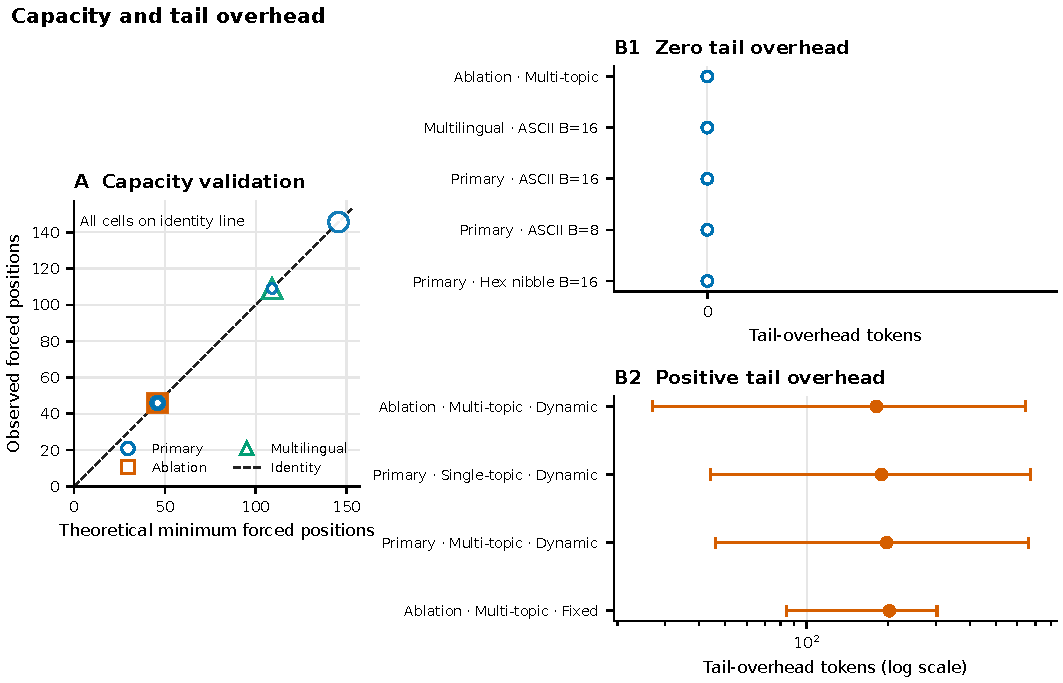
\includegraphics[width=\textwidth]{figures/capacity_tail_validation.pdf}
\caption{\label{fig:capacity}\textbf{Capacity and tail overhead.} Fixed-radix payload length and effective full-message rate are checked against their declared algebraic bounds, while the cover-length residual isolates tokens beyond the forced payload positions. Across 17,424 retained records, 7,008 were evaluable for the complete plotted capacity/quality checks; no forced-position, rate-bound, or evaluated quality-bound violation occurred. Positive residuals in 2,976 records represent natural tails or other cover overhead. Empirical agreement with these logged relationships is not evidence of human-perceived naturalness, and the complete encoder--decoder cascade cannot be reconstructed from the retained trace schema.}
\end{figure}

\subsection*{Exact-copy replay and transmission fragility}\label{sec:results-robustness}

Replay mode materially changed recovery (Fig.~\ref{fig:robustness}). Saved-token replay recovered 144/144 robustness covers, whereas detokenizing the same covers and retokenizing their visible text recovered 88/144 (0.611111). Thus, even an unedited visible string did not guarantee the original token sequence. Raw unmodified transmission recovered 144/144, but common transformations were damaging: Unicode NFKC recovered 82/144 (0.569444), quote conversion 56/144 (0.388889), and whitespace trimming 28/144 (0.194444). Markdown copy/paste and paraphrase recovered 0/144, and the two cross-model decoder outcomes for each cover recovered 0/288.

These conditions address a different question from the primary result: whether a cover can leave its saved-token record and still recreate the forced ranks. The answer depended sharply on the frozen channel definition. The saved-ID, visible-retokenization, and raw-transmission rows are distinct replay procedures and should not be pooled. Their contrast shows why the receiver contract must name the tokenization path, not merely say that the visible text was copied exactly. Cross-model zero recovery further shows that similar prompt intent does not substitute for model and tokenizer identity.

Deleting only the declared final 10\% of a message recovered 144/144 because that operation was constrained to non-payload tail tokens. It is not evidence of arbitrary truncation tolerance: removing a forced token or earlier context would change the decoded sequence. The broader matrix also showed low recovery after token or character edits and line-ending conversion (Supplementary Note S4). Limited canonicalization preserved unmodified controls but did not recover the available transformed cells, so it did not demonstrate a general mitigation.

Tail-only truncation is consequently a boundary check on the decoder definition rather than a successful error-correction result. The decoder is designed to ignore tails, so removing only tail labels should be harmless. By contrast, prefix changes and edits inside a forced span can alter a segment's initial tokenization or model history and propagate. The failed limited-canonicalization cells show that normalizing a small declared set after the fact was insufficient in this matrix; no broader mitigation is inferred.

Relative to the reviewer-requested inventory, five transformation classes were tested directly, three had only partial proxies, and three were untested. In particular, arbitrary prefix/suffix insertion, general case conversion, and general punctuation edits were not tested; line wrapping, email/markdown quoting, and sentence-boundary changes were only partially represented. First-divergence labels locate the first observed mismatch among tokenization, context, rank, or payload stages, but are descriptive and cannot by themselves establish why a transformation failed (Supplementary Fig. S1 and Supplementary Tables S7--S8).

\begin{figure}[H]
\centering
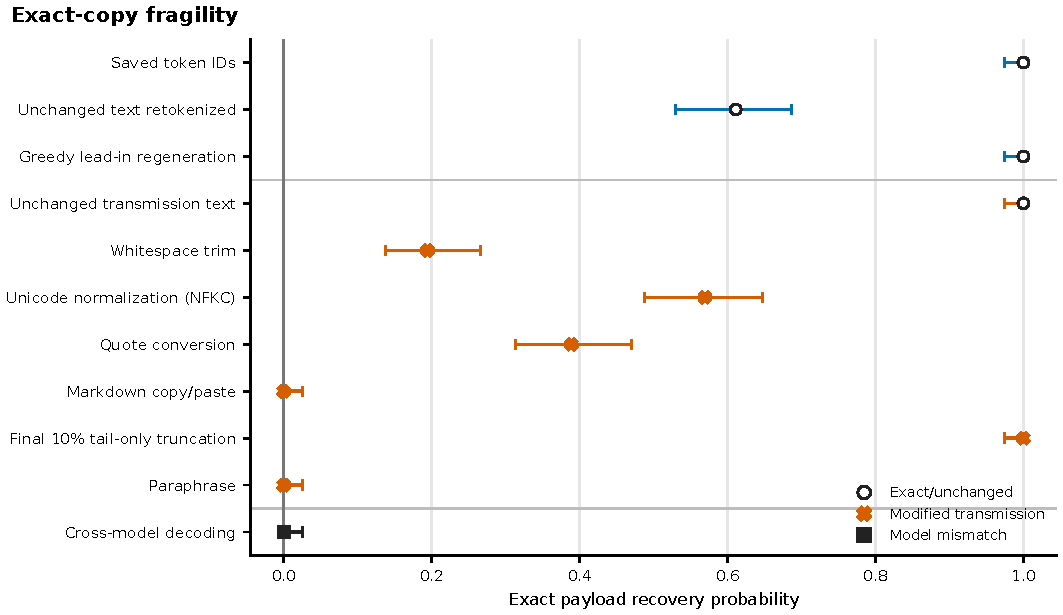
\includegraphics[width=\textwidth]{figures/robustness_recovery_compact.pdf}
\caption{\label{fig:robustness}\textbf{Exact-copy fragility.} Recovery proportions and Wilson 95\% intervals are shown for the principal replay and transmission conditions. Saved token IDs preserve the strongest replay contract; visible-text detokenization/retokenization already reduces recovery. NFKC normalization, quote conversion, and trimming reduce it further, while markdown copy/paste, paraphrase, and cross-model decoding yield no successful payloads. Final-10\%-tail truncation removes only declared non-payload tail tokens and must not be interpreted as arbitrary truncation tolerance. The full transformation matrix, denominators, limited canonicalization cells, and first-divergence diagnostics appear in Supplementary Figure S1 and Supplementary Note S4.}
\end{figure}

\subsection*{Automated readability and model-based cover quality}\label{sec:results-quality}

The balanced computational set contained 504 stimuli across seven conditions and 18 prompt templates. Ordinary controls had mean Flesch Reading Ease 61.940597 (prompt-template bootstrap 95\% CI, 54.897042--68.143167), and segmented full messages had mean 60.551834 (CI, 56.873661--64.135677; Fig.~\ref{fig:readability}). The intervals overlap substantially. Surface flags and prompt similarity supplied additional diagnostics, but none is a human rating.

The principal question was whether obvious surface diagnostics changed when bounded ranks and segmentation were used, while preserving prompt-level uncertainty. At this aggregate level, the two highlighted Flesch intervals do not show a clear separation. Flesch is driven by word, sentence, and syllable counts, however, and can assign similar scores to passages with very different coherence. Surface flags detect only declared patterns, while prompt similarity is a bag-of-words comparison. Agreement among these quantities would still not establish reader acceptance.

Source-model and held-out-evaluator log-probability contrasts did not support a universal direction of cover quality. Forty-two of 45 contrasts in each evaluator family had Holm-adjusted \(p<0.05\), yet estimates changed sign across protocol/model cells: source-model contrasts ranged from -5.298565 to +2.684536 and held-out-evaluator contrasts from -6.161972 to +3.287497. Both quality mixed models were singular, so these conditional model-scale differences require caution. The forced span also answers a different question from the full message: only the former carries ranks, while the latter includes a sometimes long greedy tail.

The large number of adjusted contrasts excluding zero therefore does not yield a single quality ranking. It instead shows protocol-by-model dependence: a cover family can score higher in one conditional evaluator cell and lower in another. Full-message scores may also be dominated by greedy tokens that the decoder discards. Reporting the forced span separately prevents fluent tail text from obscuring likelihood pressure at payload-bearing positions, but neither scale has been calibrated to human judgments.

There were zero participants and zero human ratings. Established automated metrics and prepared study materials therefore only partially address the request for human evaluation. Participant research remains uncollected and would require ethics authorization, recruitment, and deployment; the planning material is not treated as an administered survey or a result (Supplementary Table S9).

\begin{figure}[H]
\centering
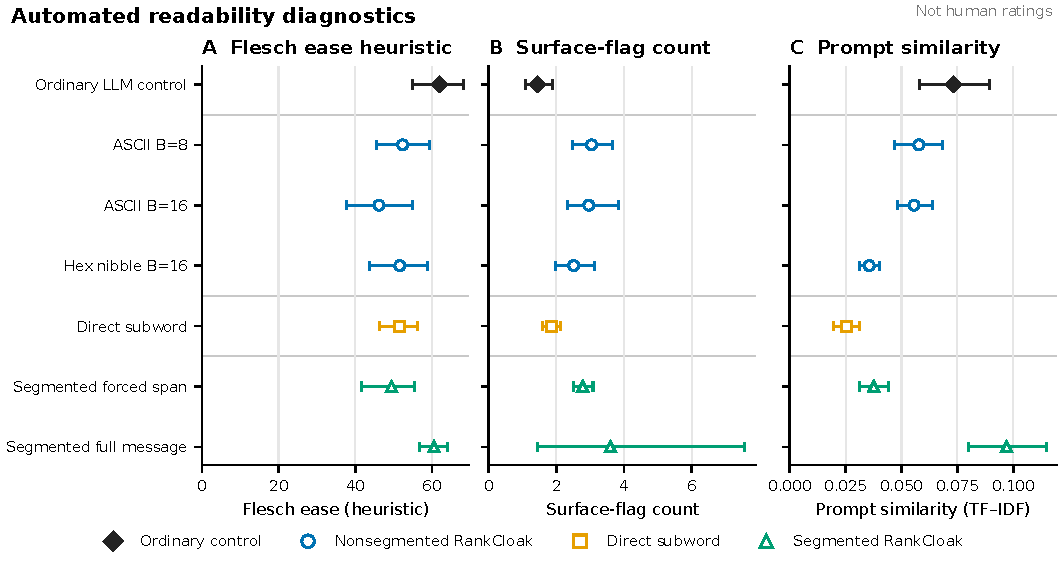
\includegraphics[width=\textwidth]{figures/automated_readability.pdf}
\caption{\label{fig:readability}\textbf{Automated readability diagnostics.} Flesch Reading Ease and related surface diagnostics are summarized over 504 balanced computational stimuli, with uncertainty resampled over prompt templates. Segmented full messages include both payload-bearing forced spans and non-payload natural tails. These measures describe surface properties of the retained text and are not human ratings, evidence of human-perceived naturalness, or substitutes for a participant study. No participant was recruited and no rating was collected. Model-based quality analyses and their singular-fit warnings are reported separately in the text and Supplementary Note S5.}
\end{figure}

\subsection*{Ablations, dynamic stopping, and prompt-topic effects}\label{sec:results-ablations}

The locked compact ablation extraction compared 48 paired payload groups across three models and is exploratory/post-outcome (Table~\ref{tab:reviewer-analyses}). A 32-token lead-in, relative to no lead-in, reduced mean log probability by 1.652327 (95\% CI, -1.749091 to -1.553103) and added 159.590278 full-message tokens (CI, 125.829861--191.030035). This adverse result is consistent with added context and boundary cost; the contrast does not prove a single failure mechanism. Increasing the segment size from 8 to 32 ranks increased effective rate by 1.231461 bits per full token (CI, 1.073116--1.388188) and reduced full length by 174.500000 tokens (CI, -208.405035 to -140.573264), trading fewer tails for longer forced spans.

The lead-in and segment results locate different costs. A lead-in precedes the forced span, consumes visible tokens, and changes the distribution used for every encoded rank; it therefore cannot be treated as a harmless stylistic prefix. Larger segments keep the forced count fixed but require fewer prompt resets and tail opportunities. Their higher effective rate is consistent with reduced overhead, while the forced span itself lasts longer before an ordinary greedy continuation begins.

Removing the safe-text filter changed mean log probability by approximately -0.0018 (canonical CSV estimate -0.001797; CI, -0.037738--0.035394) and effective rate by -0.062969 bits per full token (CI, -0.134265--0.007651); both intervals included zero. The Mistral roundtrip-stable-filter cell was unavailable for 48 work units, although the no-filter contrast included all three models. The filter results therefore do not establish a quality benefit.

The near-zero selected filter estimates are important null evidence. The deterministic filter remains necessary to define an agreed candidate set for the canonical protocol, but this ablation did not show that it improved the selected likelihood or rate endpoints. Nor can the unavailable stable-filter Mistral condition be treated as evidence for or against that condition; it is an absence caused by the frozen isolated-vocabulary criterion.

Compared with dynamic stopping, no tail increased effective rate by 3.171551 bits per full token and shortened messages by 254.951389 tokens. This arithmetic consequence of removing non-payload text is not evidence of better cover quality. A fixed 20--60-token sentence-tail policy shortened messages by 65.708333 tokens relative to dynamic stopping, whereas its selected effective-rate interval included zero. Dynamic stopping remains a declared heuristic with an emergency cap, not a semantic judgment by readers.

The tail ablation also prevents a misleading optimization conclusion. Maximizing bits per full token alone selects no tail because every added non-payload token enlarges the denominator. RankCloak introduced tails for a different, unverified purpose: allowing a forced fragment to continue to a rule-defined stopping point. Without human ratings, the experiment measures the length/rate price of that choice but cannot determine whether the price purchases perceived naturalness.

Across 15 locked topic contrasts, one Llama artifact-count comparison excluded the null: multi-topic versus single-topic expected count ratio 1.276361 (95\% CI, 1.114743--1.461409; Holm-adjusted \(p=0.003294\)). The other 14 adjusted \(p\)-values were at least 0.396248. This compact extraction was performed post-outcome without refitting models and is exploratory; it does not support a general prompt-topic advantage.

The solitary non-null row concerns one model and one artifact-count outcome. It did not recur across the other model/outcome combinations after adjustment. Accordingly, prompt diversity is retained as design coverage rather than promoted as a performance-enhancing intervention. Reviewer-relevant ablations and all topic contrasts appear in Supplementary Fig. S2 and Supplementary Tables S10--S11; the complete 60-row contrast table remains machine-readable in the public repository.

\begin{table}[H]
\centering
\scriptsize
\setlength{\tabcolsep}{2.5pt}
\begin{tabularx}{\textwidth}{L{0.13\textwidth}L{0.13\textwidth}Y Y L{0.105\textwidth}Y}
\toprule
Analysis & Sample/group & Principal estimate & Uncertainty or adjusted test & Classification & Main limitation \\
\midrule
32-token lead-in vs none & 48 paired payloads; 3 models & Mean log probability -1.652327; full length +159.590278 & CIs -1.749091 to -1.553103; 125.829861 to 191.030035 & Exploratory, post-outcome & Boundary/context interpretation is not causal \\
32- vs 8-rank segments & Same & Effective rate +1.231461 bits/full token; length -174.500000 & CIs 1.073116--1.388188; -208.405035 to -140.573264 & Exploratory, post-outcome & Fewer tails accompany longer forced spans \\
No filter vs safe filter & Same & Log probability -0.001797; rate -0.062969 & CIs -0.037738--0.035394; -0.134265--0.007651 & Exploratory, post-outcome & Both selected intervals include zero; stable-filter Mistral cell unavailable \\
Tail policy & Same & No tail: rate +3.171551, length -254.951389; fixed tail: length -65.708333 & Selected 95\% CIs in Supplementary Note S6 & Exploratory, post-outcome & Rate gain from deleting non-payload text is not quality gain \\
Topic schedule & 15 locked contrasts & Llama artifact-count ratio 1.276361 & CI 1.114743--1.461409; Holm \(p=0.003294\); other \(p_{\rm Holm}\geq0.396248\) & Exploratory, post-outcome & One selected model/outcome contrast excludes null \\
Generation overhead & 18 model--protocol cells; 12,144 matched rows & Mean 1.674368--16.087628 s; 13.631855--100.851772 bit/s & Payload-bootstrap intervals in Supplementary Note S9 & Supporting measurement & Inclusive wall time; no CPU time or warm-up repeats \\
\bottomrule
\end{tabularx}
\caption{\label{tab:reviewer-analyses}\textbf{Compact reviewer-requested analysis and operational summary.} Differences are level minus canonical unless otherwise stated. Ablation and topic rows are a locked exploratory/post-outcome extraction from retained analyses; no new model was fit. Reviewer-relevant ablations, complete topic rows, availability, and timing cells are in the Supplementary Information; the full 60-row contrast table remains machine-readable in the repository.}
\end{table}

\subsection*{Neural steganalysis}\label{sec:results-detector}

Both classifiers strongly separated RankCloak covers from matched controls (Fig.~\ref{fig:detector}). TextCNN matched ROC-AUC was 0.990190 (payload-group bootstrap 95\% CI, 0.987740--0.992682) with balanced accuracy 0.951010 (CI, 0.943456--0.958466). DeBERTa-v3-base ROC-AUC was 0.999834 (CI, 0.999696--0.999939) with balanced accuracy 0.991919 (CI, 0.987654--0.995665). High performance is adverse evidence for concealment, not a security feature of RankCloak.

This test directly challenges the premise that removing visible artifact syntax is sufficient for concealment. The corpus was balanced between RankCloak and matched ordinary controls and split by payload group, so the matched estimates cannot be attributed to class imbalance or row-level payload leakage. Both a compact convolutional model and a pretrained transformer found strong signal. The evidence is limited to this constructed corpus and training procedure, but within that scope it contradicts any claim of practical undetectability.

Generalization depended on architecture and split. Across 18 held-out templates, TextCNN ROC-AUC ranged 0.720421--0.981705 and balanced accuracy 0.565909--0.919318; DeBERTa ranges were 0.996291--0.999979 and 0.952273--0.995455. Leave-one-model ROC-AUC ranges were 0.925623--0.973650 for TextCNN and 0.996772--0.999979 for DeBERTa; leave-one-codec ranges were 0.966532--0.998634 and 0.997917--1.000000. These are ranges across distinct held-out splits, not confidence intervals for one pooled estimate.

The TextCNN template range shows meaningful distribution sensitivity: a high matched score alone does not specify behavior for every new prompt. DeBERTa remained near perfect over the evaluated held-out regimes, which strengthens the adverse conclusion for these model, prompt, and codec families. It still does not establish performance on arbitrary human text, unseen generation systems, or future RankCloak modifications. The ranges deliberately preserve heterogeneity instead of averaging unlike test sets.

Exact text-identity and token-sequence leakage checks passed for all 28 frozen splits. A stricter lexical diagnostic nevertheless found 53 normalized near-duplicate pairs at the declared threshold, including 44 cross-payload pairs, affecting 16 splits. Excluding affected test payload groups without retraining changed ROC-AUC by -0.001925 to +0.004568 for TextCNN and -0.000038 to +0.000166 for DeBERTa; balanced-accuracy changes were similarly small. This sensitivity does not remove the design limitation because it is diagnostic, threshold-dependent, and does not rebuild the training sets. Fixed-seed repetition on the same CUDA device reproduced scores exactly for both architectures. It supplies same-device repeatability only; no CPU/GPU equivalence experiment was completed.

Small exclusion deltas show that the observed metrics were not numerically overturned by this particular thresholded removal, but they cannot prove independence of lexical structure. The sensitivity discarded affected test payload groups after training and did not reconstruct all split assignments. Supplementary precision, Brier score, and low-false-positive sensitivity are likewise labeled exploratory. Same-device exact repetition verifies the saved CUDA procedure, not portability across processor types (Supplementary Fig. S3 and Supplementary Tables S12--S13).

\begin{figure}[H]
\centering
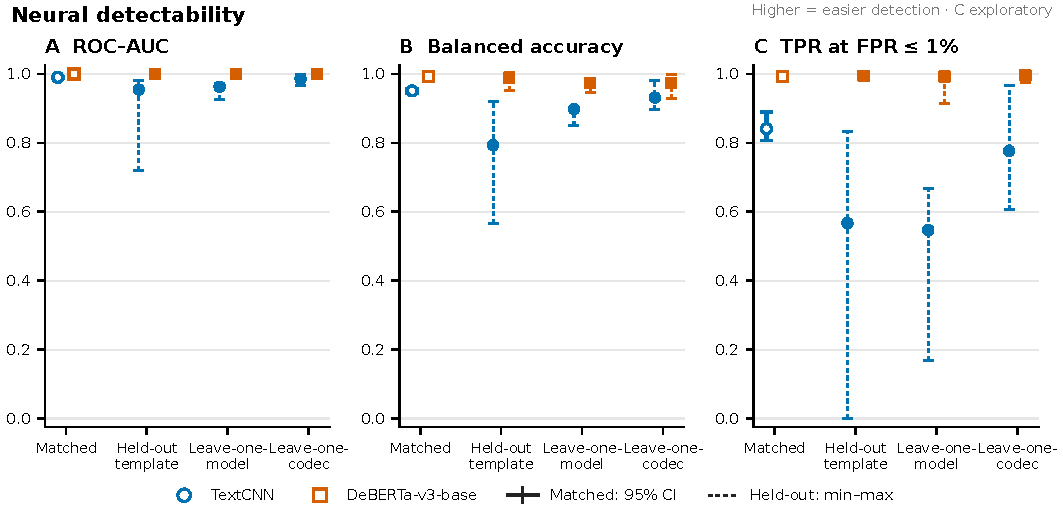
\includegraphics[width=\textwidth]{figures/neural_detector_performance_compact.pdf}
\caption{\label{fig:detector}\textbf{Neural detectability.} Matched ROC-AUC and balanced accuracy are shown with payload-group bootstrap 95\% confidence intervals; held-out-template, leave-one-model, and leave-one-codec results are summarized as ranges across frozen splits. Higher performance is adverse for RankCloak concealment because it indicates that covers are distinguishable from matched controls. Both classifiers completed all 28 regimes. Exact identity leakage checks passed, but a declared lexical near-duplicate diagnostic affected 16 splits; exclusion sensitivity produced small observed changes without eliminating that limitation. The full six-panel view and exploratory precision, Brier, low-false-positive, leakage, and repeatability results appear in Supplementary Figure S3.}
\end{figure}

\subsection*{Computational overhead and generalizability}\label{sec:results-overhead}

Across the 18 primary model--protocol cells, mean inclusive generation time ranged from 1.674368 to 16.087628 seconds. Mean payload throughput ranged from 13.631855 to 100.851772 bits/s, and effective rate from 0.710004 to 7.322003 bits per full token. These saved wall times include wrapper setup and decoding scope defined by the harness; CPU time and repeated warm-up measurements were not retained.

The approximately order-of-magnitude spread across cells shows that representation and model choice materially affect operational cost in the retained environment. Compact direct ranks can reduce forced work, whereas byte expansion and repeated segmented continuations increase it. Throughput and effective rate answer different questions: the first normalizes payload bits by wall time, while the second normalizes by visible full-message tokens. Neither is a deployment benchmark outside the recorded wrapper and device.

On the fixed CUDA benchmark, representative TextCNN wall/training times were 91.358/9.498 seconds with 306.25 MB peak allocated VRAM; DeBERTa-v3-base times were 1,536.661/1,425.063 seconds with 6.38 GB. Those device-specific measurements do not generalize across hardware. Evaluation across three model families and exact-copy Spanish and Simplified Chinese trials broadens the controlled design, but does not validate very-large proprietary models, broad multilingual cover quality, operational channels, or real-world deployment.

The detector timings also illustrate the cost of the stronger adverse test: the pretrained architecture required substantially more saved time and memory than TextCNN in the single retained benchmark. CPU neural training was infeasible and was not used as a comparison point. These measurements support transparent study accounting, not a claim that the approach is efficient enough for an operational sender, receiver, or monitor (Supplementary Fig. S4 and Supplementary Tables S15--S16).

\section*{Discussion}\label{sec:discussion}

RankCloak provides a reproducible method for converting serialized cryptographic artifacts into language-model next-token ranks and measuring the cover text that realizes them. Its representation choices expose a central trade-off. Direct subwords can be compact but leave rank pressure uncontrolled, whereas ASCII-byte and hex-nibble codecs bound the permitted rank by spending more forced positions. Segmentation redistributes those positions across contexts, and natural tails add non-payload length. The formal and empirical capacity relationships make these costs explicit rather than treating longer cover text as additional payload capacity.

Complete recovery in the evaluated primary and secondary-language matrices establishes deterministic codec and replay fidelity under the saved-token exact-copy contract. It does not establish an ordinary text channel. Detokenized visible text could change tokenization without an apparent edit, and common normalization, formatting, rewriting, or model-mismatch conditions sharply reduced or eliminated recovery. The contrast between perfect saved-token replay and fragile visible-text transmission is therefore not a secondary implementation detail; it defines the boundary of the recovery claim.

Cover-quality evidence was mixed and protocol-dependent. Aggregate automated readability values for ordinary controls and segmented full messages were similar, while source-model and held-out-evaluator contrasts changed direction across model and protocol cells. Forced spans and full messages also measure different mixtures of payload pressure and greedy continuation. These diagnostics help compare mechanisms, but they are not equivalent to human evaluation, and no participant evidence supports a claim of human-perceived naturalness.

Supporting analyses reinforce this interpretation without identifying a single optimum. Larger segments improved efficiency by reducing repeated tail overhead, while lead-ins worsened likelihood and length in the selected contrasts; removing tails mechanically improved rate but did not test perceived quality. These exploratory comparisons show that optimization depends on which cost is prioritized rather than establishing a universally preferable protocol. Evaluation across three model families, diverse prompts, and two secondary languages broadens the controlled setting, but cannot be extrapolated to arbitrary models, languages, or deployed channels.

Neural steganalysis supplies the clearest adverse finding. Both detector architectures achieved very high matched performance, and the pretrained detector remained highly effective across the evaluated held-out regimes. Although split sensitivity and lexical overlap limit extrapolation, the observed distinguishability directly argues against practical concealment in this corpus. Exact recovery cannot compensate for a cover distribution that trained classifiers can identify with near-perfect accuracy.

Despite these adverse results, the study contributes a controlled framework for separating representation, recovery assumptions, capacity, cover length, automated quality, transformation sensitivity, and detectability. The expanded payload, prompt, model, and secondary-language design shows how these quantities can be evaluated without equating model likelihood with reader judgment or deterministic replay with channel robustness. RankCloak therefore establishes a measurement framework and a set of reproducible failure surfaces for rank-based hiding; it does not establish a secure, undetectable, robust, or deployment-ready covert communication system.

\section*{Responsible use and limitations}\label{sec:limitations}

RankCloak is dual use and can encode sensitive-looking artifacts, but it does not itself provide encryption, authentication, confidentiality, or a cryptographic-security proof; any protected payload still requires an external cryptographic system and an explicit threat model. Exact recovery depends on saved-token replay, whereas visible-text transmission and common transformations are fragile and the tested perturbations do not establish broad edit robustness. Human-perceived naturalness, broad multilingual behavior, real-world deployment, and performance across arbitrary future models or communication channels were not established; automated measures are not participant ratings, and detector performance is limited to the evaluated corpus. The evidence therefore supports RankCloak as a controlled research framework, not as a secure, undetectable, robust, or deployment-ready covert channel; detailed boundaries appear in Supplementary Table S17.

\section*{Data and Code availability}\label{sec:data-code}

The RankCloak source code and computational data supporting this study are available at the GitHub repository, \url{https://github.com/mantzaris/llm-rankcloak}, and are archived in Zenodo at \url{https://doi.org/10.5281/zenodo.21987450}. The archive contains the public payload corpus, analysis inputs, detector predictions and metrics, source tables, figures, configurations, and provenance required to inspect the reported computational results.

\bibliography{references}

\section*{Acknowledgements}

None.

\section*{Author contributions}

A.V.M. conceived the study, developed the methodology and software, conducted the original computational work, curated and interpreted the evidence, and is responsible for the manuscript.

\section*{Funding}

No specific funding was reported.

\section*{Competing interests}

The author declares no competing interests.

\end{document}
